\chapter{Problem Statement}

From the beginning of civilization, humans have been looking to transport from one place to another more efficiently than walking. First, they start with horses and floats, but horses had a brain and could make its own decisions; sometimes, those decisions were based on an emotional reaction rather than intelligent choices. Moreover, it could not continuously work for a long duty cycle, and its power was limited. Later in 1769, Nicolas-Joseph Cugnot invented the first steam-powered vehicle. This incredible machine could load an extended amount of weight, and drivers could make their own driving decisions. Until now, this transportation system is still working; unless the advantage of efficiency, power consumption, pollution, and safety is not enough to be an optimal way to transport people and loads.\\

Research areas have made many efforts to achieve an optimal way of transportation to be accessible, optimal, and safe for everybody. Some ideas have been proposed, like hydrogen, diesel, and natural gas engines. Also, some Nobel research about control safety systems like better and more powerful breaks, automated airbags, and good chassis material try to save more lives, but it is not enough. Unfortunately, all past advantages are focused on the driver and the users of the vehicle. Currently, there is not any control system that warranty the security and integrity of the other road authors in the way. The human decision in a driving context frequently represents a danger because it is based on emotion and natural reaction making no optimal driving. Even though these options could improve the current vehicles, they may find a better and cheapest solution to the main problem.\\

The research areas try to solve the safety driving problem with DeepLearning, Recurrent Neural Networks, machine learning, etc. However, using these theories does not warranty stability and controllability in all possible scenarios. To get a closer solution to this specific problem, we study one way of achieving security and efficiency in a particular method as a highway area in this thesis work. Currently, the experts on optimal control system areas rely on automated driving. This technology could solve all of the problems mentioned above.\\

Some safety decision criteria that we take into account were the following:
\begin{itemize}
\item Avoid obstacles that may be on the road.
\item Avoid a collision with other cars in the road regardless of whether it is a cooperative or non-cooperative agent.
\item Make decisions in the presence of aggressive maneuvers by selfish or non-cooperative agents on the road.

\end{itemize}


Therefore, it was necessary to design and implement different controllers with access to specific data sets. It depends on each controller's necessity. These decisions are based on a logical and optimal decision-maker control to achieve the desired goal.

 These decisions are based on safety rules established for the users for any particular road.


% --------------------- automated driving --------------------
\section{Automated driving}
The idea in automated driving job is to achieve coordination and synchronization of several autonomous vehicles (AV) safely and efficiently.\\

To manage a massive number of  AV requires an extensive network with high computational loads and advanced control techniques. Usually, in the research literature is implemented one control algorithm for an agent to achieve the objective. However, automated driving is an area that must consider different scenarios and situations. Besides, it is essential to prove all possibilities for warranty security and entirely controllability. This thesis studies some control theories and the best state to implement.

\begin{itemize}
    \item  \textbf{Mixed-Integer Potential Game:} uses integer and continuous variables in a cost function to control the AV's position and velocity on a highway optimally.
    \item  \textbf{Model Predictive Control:} uses information about the environment and local variables to get the optimal decision avoiding near obstacles.
    \item  \textbf{Alternating Direction Method of Multipliers:} utilize a linear model of the AV and inequality constraints as possible to get a faster and more efficient solution to the problem. 
\end{itemize}

All the above controllers are explained in detail in chapter 4. In addition, the following section describes how the AV and the collision avoidance are modeled. 






% -----------------------------------------
\section{Vehicle Modelling}

The automated driving task is a complex job, and one model is not enough to represent the behavior of a vehicle around the environment. However, multiple controllers require multiple models that give the correct information. We use three different controllers that have a specific task. Each of them needs a particular model of a vehicle. The high-level controller takes the network's information. For that reason, we implement a linear model. The middle-level controller uses just the knowledge of the environment acquired by its sensors. Due to this reason, we implemented a unicycle model. Besides, the low-level control gets information about the car and its behavior to make decisions. Thus, we use a differential model in this control section. 


% -----------------------------------------
\subsection{Linear Model System}
For controllers based on game theory, convexity is the main prerequisite for convergence. Therefore, the robot model and its constraints need to be linear and convex. Due to this, the system is based on a Mixed-Logical-Dynamical system \cite{BEMPORAD1999407}. We consider a set of vehicles $\mathcal{I}:= \left \{ 1, ..., N \right \}$ where N is the total number of vehicles interacting with the local agent on a multi-lane environment. The set  $\mathcal{L}:= \left \{ 1, ..., L \right \}$, represents the set of current lines on the highway, L is the maximum number of lines on the way. We assume that each vehicle $i$ can control its longitudinal speed $v_i \in \mathcal{V}_i \subset \mathbb{R}$  and can change lane $z_i \in \mathcal{L} \subset \mathbb{N}$. Over the prediction horizon $\mathcal{T} := \left \{ 0, ... ,T \right \} , T\geq 1$. We use two different decision variables to better represent an AV on a highway. Mixed logical variables can simplify, make linear, and convex the entire system. 

\begin{figure}[H]
    \centering
    \includegraphics[width=0.8\textwidth]{Kap3/linear_model.png}
    \caption{Linear model's variables}
    \label{fig:variables}
\end{figure}


\subsubsection{Continuous Decision Variables}
Each vehicle model has continues variables that represent some physical features. Longitudinal acceleration $a_i \in A_i := \left [ \underline{a_i}, \overline{a_i} \right ] \subset \mathbb{R}$, the variables $\left \{ \underline{a_i}, \overline{a_i} \right \}
$ represent the minimum and maximum acceleration allowed, with $\underline{a_i}< 0 <  \overline{a_i} $, assuming that the $\underline{a_i}$ is negative and is due the break job of the $i$ vehicle, as illustrated in Fig. \label{fig:variables}. The longitudinal speed $v_i \in \mathcal{V}_i \subset \mathbb{R}$ is determined by a standard Forward-Euler Scheme, i.e.,

\begin{gather}
v_i(t+1) = v_i(t) + \tau a_i(t),
\end{gather}

where $\tau > 0$ denotes the time interval of each simulation step. Hence, the acceleration and velocity longitudinal over the horizon $\mathcal{T}$ are: 
\begin{gather*}
a_i := \left [ a_i(0); ...; a_i(t-1) \right ] \in \mathcal{A}^T_i, \\
v_i := \left [ v_i(0); ...; v_i(t-1) \right ] \in \mathcal{V}^T_i
\end{gather*}




\subsubsection{Discrete Decision Variables}
The lanes in a highway are predefined internationally as a space where the vehicles can and should travel. Because of this design, a rule recommends driving inside a lane unless the vehicle needs to change to another one. That means the set of vehicles $\mathcal{V}$ needs to be modeled as an integer variable that represents the actual and future traveling lane $z_i \in \mathcal{L}$. The discrete decision variables over the horizon $\matchal{T}$ are:

\begin{gather*}
z_i := \left [ z_i(0); ...; \z_i(t-1) \right ] \in \mathcal{Z}^T_i.
\end{gather*}



\subsubsection{Coupling Variables}



The control system requires different sense variables that allow knowing the actual and future states of the agent $i$ with its neighbors $\mathcal{I}_{-i}$. Therefore, we denote by $d_{i,j} \in \mathbb{R}$ as the longitudinal distance between the connected vehicles $i$ and $j$ at the time $t \in \mathcal{L}$ as shown the Fig. \label{fig:variables}. The behavior of $d_{i,j}$ over time evolves as a Forward-Euler function:

\begin{equation}
d_{i,j}(t+1)= d_{i,j}(t) + \tau(v_j(t)-v_i(t)).
\label{eq:distance}
\end{equation}

\begin{figure}[H]
    \centering
    \includegraphics[width=0.5\textwidth]{Kap3/Asset 4.png}
    \caption{Relative distance between agents.}
    \label{fig:distance}
\end{figure}



It allows us to introduce the set of vehicles in the neighborhood of  $\mathcal{N}_i := \left\{ j \in \mathcal{I}  | \left| d_{i,j} \right| \le \overline{d} , t \in \mathcal{T}\right\}$; this data can be measured locally or globally example, on the on-board sensors or with communication of a driving network. From now we refer to the variable $j$ as a generic vehicle in the set $\mathcal{N}_i$. According to \label{eq:distance}, each agent knowing the velocity of its neighbor $v_j(t)$, can estimate the relative distance between each other.
In addition, we implement a relative lane distance $z_{i,j}$. It represent the difference of lane between agent $i$ with its neighbors $\mathcal{N}_i$ and is represented by the following equation:

\begin{equation}
z_{i,j}(t)= z_{j}(t) + z_{i}(t).
\label{eq:lanes}
\end{equation}

\begin{figure}[H]
    \centering
    \includegraphics[width=0.6\textwidth]{Kap3/Asset 5.png}
    \caption{Difference of lane.}
    \label{fig:lanes}
\end{figure}

We assume that each agent makes decisions for their selfish interest, e.g., drive through desired speed profile $v_i^d \in \mathcal{V}^T_i$ or get into a lane $z_i^d \in \mathcal{L}^T_i $. The control system of each agent takes into account the current and future state of its neighbors. Still, he gets no information about the targets of the other agents. As a result of this behavior, each agent takes decision seeking its individual goals through a sequence of hybrid decisions.
With the previous model, we formulate as a first step a Model Predictive Control (MPC) motion planning with mixed-integer variables:

\begin{gather}
    \left\{ \begin{array}{cl}
 \min_{v_i, a_i, z_i} J_i(v_i, a_i, z_i) & \\
\text{s.t.} \quad v_i(t+1)=v_i(t)+ \tau \ a_i(t), & \forall t \in \mathcal{T} \\
a_i(t) \in \mathcal{A}_i,  & \forall t \in \mathcal{T} \\
v_i(t+1) \in \mathcal{V}_i,  & \forall t \in \mathcal{T} \\
z_i(t+1) \in \mathcal{L}_i,  & \forall t \in \mathcal{T} \\
\end{array} \right.
\label{eq:MPC1}
\end{gather}
\\
The $J_i$ cost function is a linear and convex objective for each vehicle $i$ where $J_i:\mathcal{V}^T_i \times \mathcal{A}^T_i \times  \mathcal{L}^T_i \longrightarrow  \mathbb{R}$. The sets $\mathcal{V}_i$ and $\mathcal{L}_i \subset \mathcal{L}$ shall be defined to restrict them to possible values in the real environment. Given maximum and minimum acceleration $\left[ \underline{a_i}, \overline{a_i} \right]$ as also maximum and minimum Velocity $\left[ \underline{v_i}, \overline{v_i} \right]$, we can limit the sets as:

\begin{align}
    \mathcal{V}_i(t) & :=\left[ 0,\overline{v_i(t)} \right] \cap \left[ v_i(t)+ \tau  \underline{a_i},\quad v_i(t)+ \tau  \overline{a_i} \right]
    \label{eq:set_v}
\\
    \mathcal{L}_i(t) & :=\mathcal{L} \cap \left[ z_i(t) -1, \quad z_i(t)+1 \right]
    \label{eq:set_z}
\end{align}

From \ref{eq:set_v} its possible to limit the speed to legally possible values, and from \ref{eq:set_z} limits the change of lane just one per step. This restriction makes agents' movement smoother through lanes and makes possible lateral safety rules. The following section explains the rules to make safer automated driving with selfish agents.

\subsection{Collision Avoidance Rules}
 
Human driving is usually unsafe; there are some rules established in each country, like speed limits, preferential lanes, and safety distance. In this section, we postulate some safety rules to avoid the collisions of the interconnected agents with the presence of non-cooperative agents.\\

% -----------------------------------------------------------------------------
\subsubsection{Longitudinal rules}
the main reason for a collision of two or more vehicles is that one of them breaks the safety distance. Due to this is implemented the following safety rule. If the lateral distance between two agents is equal to zero $z_j(t)=z_i(t) $ and the longitudinal distance is greater or less than a safety distance $\left| d_{i,j}(t) \right| > D_s$, and the agents will continue in the same lane $z_i(t+1) =  z_i(t), z_j(t+1) =  z_j(t)$, the control system must ensure that the behind vehicle maintains a safety distance $\left| d_{i,j}(t) \right| > D_s$ how is shown in Algorithm \ref{alg:safety}, where $D_s$ is a predefined secure distance.\\

\begin{algorithm}
\caption{Algorithm of longitudinal distance}\label{alg:safety}
\begin{algorithmic}
% \FOR $i \in \mathcal{V}$
% \FOR \forall {$i \in \mathcal{V}$} 
\If{$z_{i,j}(t)=0$ and $z_{i,j}(t+1) =0$}
    \If{$d_{i,j}(t) > 0 $}
        \State $d_j(v_j(t)) -d_i(v_i(t)) > D_s$
    \ElsIf{ $d_{i,j}(t) < 0$} 
        \State $d_j(v_j(t)) -d_i(v_i(t)) < -D_s$
    \Else
        
        \State Continue normal driving
    \EndIf
\EndIf

\end{algorithmic}
\end{algorithm}

% ----------------------------------------------------------------------------
\subsubsection{Lateral rules}

\begin{figure}
\begin{subfigure}
\centering
    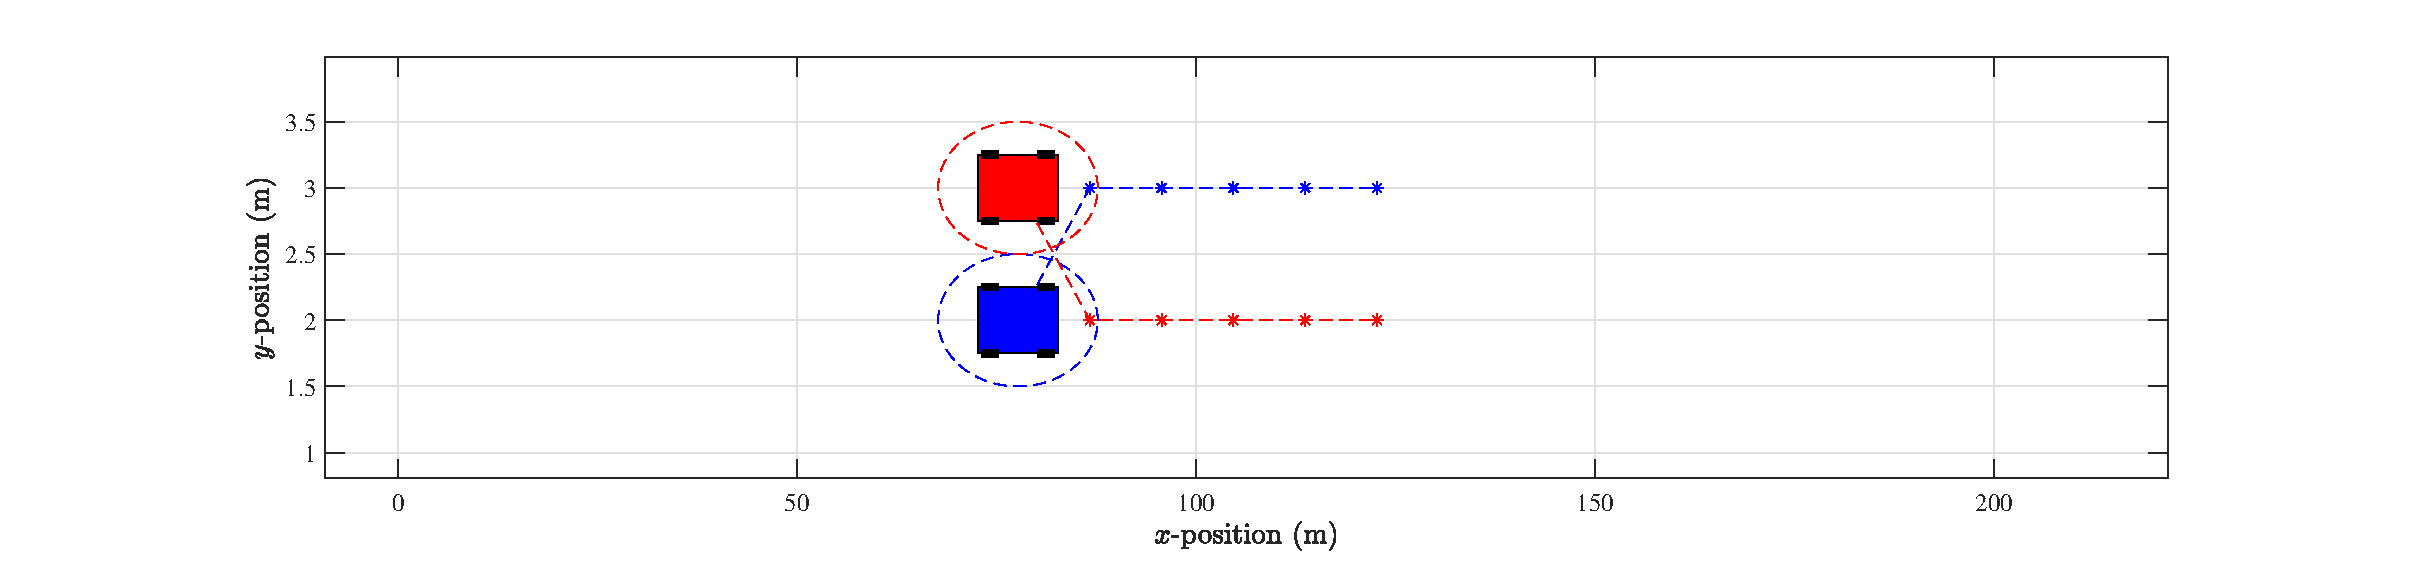
\includegraphics[width=0.9\textwidth]{Kap3/untitled.eps}
    \label{fig:lat_col1}
% \end{center}
\end{subfigure}%
\begin{subfigure}
\centering
    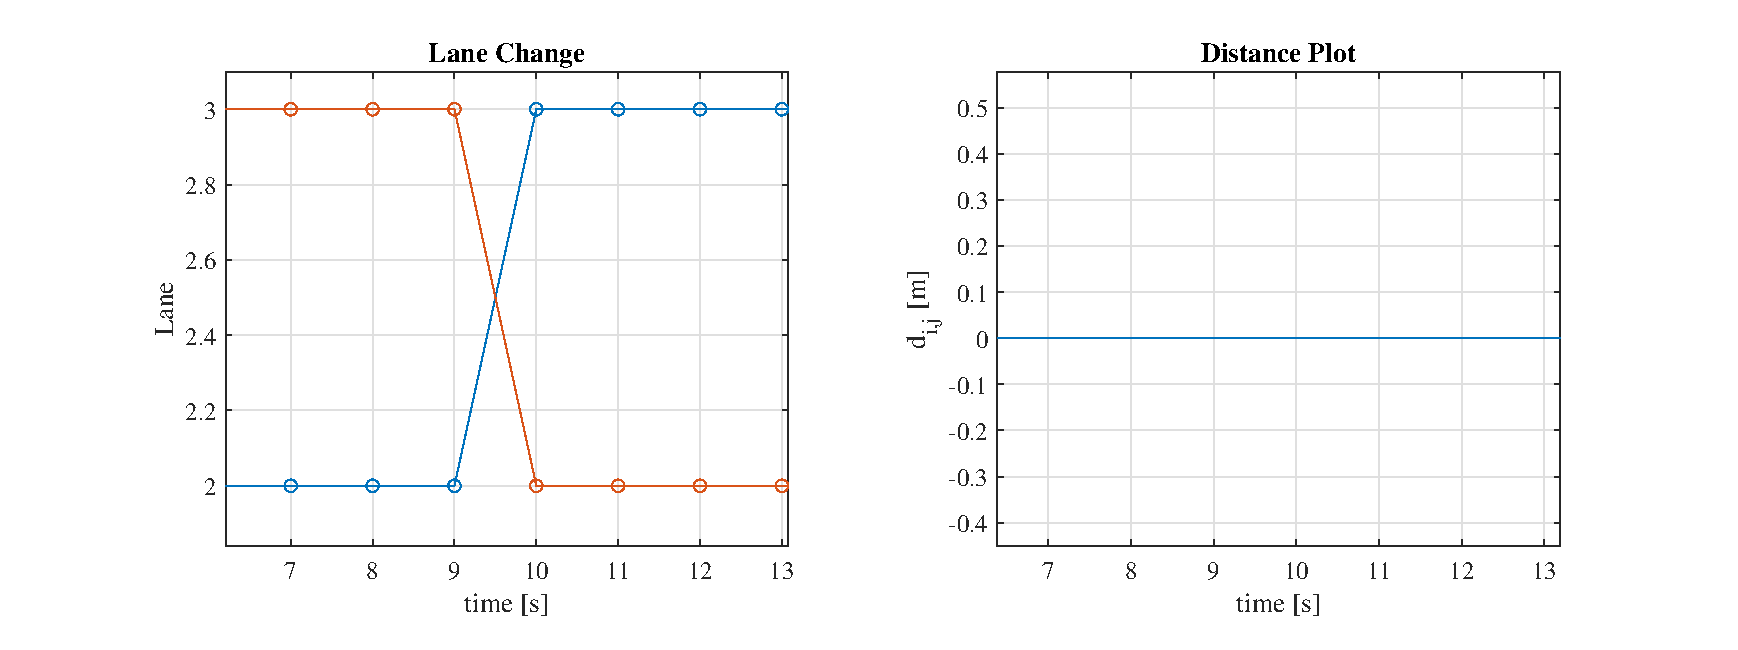
\includegraphics[width=0.9\textwidth]{Kap3/plot_change_line.eps}
    \label{fig:lat_col2}
% \end{center}
\end{subfigure}%
\caption{Lateral collisions.}
\label{fig:lat_col}
\end{figure}

There are other common collisions in a regular lane; those are lateral collisions, usually generated by occlusion problems. Thanks to interconnected and full neighbor position knowledge, this model do not have this issue. However, the controller solver could be in a position where each vehicle decide to change at the same time the lane as Fig \ref{fig:lat_col} shows. Owing to this, we implement the lateral rule for each vehicle $i,j$ driving over the horizon $\mathcal{T}$, if the longitudinal distance $d_{i,j}$ is less than a safe distance and the difference of lane position $z_{i,j}$ is one $\left| z_{i,j} (t) \right|=1$, and the pair of agents will change the lane $z_{i} (t+1) \neq z_{i} (t), z_{j} (t+1) \neq z_{j} (t)$, the controller must constraint the change of lane as is explained in the next algorithm.

\begin{algorithm}
\caption{Algorithm of lateral distance}\label{alg:lat_saf}
\begin{algorithmic}
% \FOR $i \in \mathcal{V}$
% \FOR \forall {$i \in \mathcal{V}$} 
\If{ $\left| z_{i,j} (t) \right|=1$ and ($z_{i} (t+1) \neq z_{i} (t)$ or $ z_{j} (t+1) \neq z_{j} (t)$)}
    \If{$d_{i,j}(t) > 0 $}
        \State $d_j(v_j(t)) -d_i(v_i(t)) > D_s$
    \ElsIf{ $d_{i,j}(t) < 0$} 
        \State $d_j(v_j(t)) -d_i(v_i(t)) < -D_s$
    \Else
        
        \State Continue normal driving
    \EndIf
\EndIf

\end{algorithmic}
\end{algorithm}

Finally,  the previous safety rules are executed in a mixed-integer decision-making framework explained the in-depth way in chapter \ref{Unicicle_model}. Nevertheless, this thesis work does not focus on the issue of communication among vehicles. Consequently, we assume that:
\begin{itemize}
    \item vehicles can share data of their position, speed, current lane and future states planned. 
\item each vehicle is autonomously, therefore it has the capability of change its position and velocity without the presence or intervention of a human being
\end{itemize}







% ##############################################
\subsection{Unicycle Model System}
\label{Unicicle_model}
We use a unicycle model to represent the kinematics of each vehicle \cite{kinematic}. This model is usually described by a simple non/linear model: 


% \begin{equation}
\begin{align}
  \dot{x} =& v \cos{\theta}\\ 
  \dot{y} =& v \sin{\theta} \\
\dot{\theta} =& \omega  \\ 
\dot{v} =& \frac{R}{2m} (F_{r} + F_{l}) \\ 
\dot{\omega} =& \frac{R}{L \cdot I} (F_{r} - F_{l})  
\end{align}
% \end{equation}

where $x,y$ are the position in the map and $\theta$ correspond to the orientation in the world reference. Let $v, w$ be the linear and angular velocity inputs, respectively. In Fig. \ref{kinematic2} is possible to see the representation of the mentioned variables


\begin{figure}[h!]
\centering
    \includegraphics[width=0.6\textwidth]{Kap3/kinematic.png}
    \caption{Kinematic model of a differential robot.}
    \label{kinematic2}

\end{figure}


\begin{equation}
\begin{bmatrix}
w_{r}\\ w_{l}
\end{bmatrix} =  \frac{1}{2R}\begin{bmatrix}
2 & -L\\ 
2 & L
\end{bmatrix} \begin{bmatrix}
v\\ w
\end{bmatrix}.
\label{dif_equat}
\end{equation}

The robot uses a differential model in the low-level control architecture. This model allows calculating the control action in each wheel. In equation \eqref{dif_equat}, it is possible to see the math calculus to obtain the wheel velocity, where $w_{r}$ and $w_{l}$ are angular velocity of right and left wheels, respectively $L$ is the distance between the two wheels, and $R$ is the radius of both wheels. 


In many applications is important to use a basic model. this in order to make easier processing and solution of optimization algorithms. n 

The main of this model is to get information of the vehicle, and the environment like a interconected system could take them. Taking into account this we formulate an scenario where exist $L$ lanes. the vehicle can travel for each lane  



% -----------------------------------------
\subsection{Differenial Model}

% {\color{red} Esta muy floja esta parte, siga escribiendo basese de buenas referencias, por ejemplo el capítulo 13 de (Planning algorithms- Steven M. LaValle) particularmente 13.1.2 Kinematics for Wheeled Systems }






